\section{Design af filter}\label{sec:design_filter}
    Parametre som brugeren skal kunne justere: Centerfrekvensen $\omega_0$,  forstærkning $G$,  filterets godhed $Q$ som bla. beskriver båndbredden på pasbåndet.\\
    Øvrige parametre:
    $G_0$ er reference forstærkning (sættes til 1 for at kunne kaskadekoble flere bånd) og $G_B$ som er forstærkning ved knækfrekvenserne (typisk 3dB over/under fra analog filterteori).s

    \subsection{Analog filter}

	Som filter til equalizeren anvendes high-shelf, low-shelf og  peak/notch.
    Der bliver kun anvendt 2. ordens filtre, da der ikke er brug for højere orden inde for audio. 

     \subsection{Peak/notch filter}

    Et peak/notch filter i en parametrisk equalizer består af et båndpas- $H_{BP}$ og et båndstop $H_{BS}$ filter. 
    Et analogt båndpas filter kan beskrives med ligning \ref{eq:iir_bandpas} 
    hvor $\alpha$ er en konstant der er afhængig af frekvensspecifikationer, $\Omega_0$ er centerfrekvensen.\\
    I ligning \ref{eq:iir_bandstop} er en overføringsfunktion for et båndstopfilter.
    I ligning \ref{eq:iir_peaknotch} summeres båndstop- og båndpasfilteret for at kunne forstærke eller dæmpe signalet omkring center frekvensen.
    
     \begin{align}
     H_{NOTCH}(s) &= \dfrac{s^2 + \Omega_0^2}{s^2 + \alpha s + \Omega_0^2}
     \label{eq:iir_bandpas} \\
     H_{PEAK} (s) &= \dfrac{\alpha s}{s^2 + \alpha s + \Omega_0^2}  
     \label{eq:iir_bandstop} \\
     H_a (s) &= G_0 H_{NOTCH} (s) + G H_{PEAK} (s) = \dfrac{G_0 (s^2 + \Omega_0^2) + G \alpha s}{s^2 + \alpha s + \Omega_0^2}
     \label{eq:iir_peaknotch}
    \end{align}
    Filterets gain kan bestemmes ud fra ligning \ref{eq:iir_gain}.
    \begin{align}
        G_B = \dfrac{G_0^2 + G^2}{2} \label{eq:iir_gain}
    \end{align}

    Ved at sætte $s = j \Omega$ i ligning \ref{eq:iir_bandpas} og \ref{eq:iir_bandstop}, og sætte $\big| H(j\omega)\big|^2 = G_B^2$, hvor $G_B^2$ er den ønskede forstærkning ved den ønskede centerfrekvens $\Omega_0$, kan parameteren $\alpha$ findes for de givne specifikationer.

\husk{Til Dennis}{Forklarende tekst herunder}    
    \begin{align}
     |H_{a}(j \Omega)| = \dfrac{G_0 (\Omega_0^2- \Omega^2)+ j G \alpha \Omega}{-\Omega^2 + j \alpha \Omega + \Omega_0^2}   
    \end{align}

    \begin{align}
        |H_{a}|^2 = G_B^2 =  \dfrac{(\Omega_0^2- \Omega^2)^2 + G^2 \alpha^2 \Omega^2}{(\Omega_0^2-\Omega^2)^2 +\alpha^2 \Omega^2}   \iff \Omega^4 - \left(2 \Omega_0^2 + \dfrac{G^2- G_B^2}{G_B^2- G_0^2} \alpha^2 \right) \Omega^2 + \Omega_0^4 =0
    \end{align}
    
    
    \begin{align}
       \Delta \Omega^2 = (\Omega_2 - \Omega_1 ) = \dfrac{G^2 - G_B^2}{G_B^2 - G_0^2}  \alpha^2 \rightarrow \Delta \Omega = \sqrt{\dfrac{G^2 - G_B^2}{G_B^2 - G_0^2}} \alpha \iff \alpha = \sqrt{\dfrac{G_B^2-G_0^2}{G^2 - G_B^2 }} \Delta \Omega
    \end{align}


    \begin{align}
    \alpha \equiv \beta (1 + \Omega_0^2)  = \sqrt{\dfrac{G_B^2-G_0^2}{G^2 - G_B^2 }} \left( 1 + \Omega_0^2 \right) \tan \left( \dfrac{\Delta \omega}{2} \right) \\
    \iff \beta = \sqrt{\dfrac{G_B^2-G_0^2}{G^2 - G_B^2 }} \tan \left( \dfrac{\Delta \omega}{2} \right) \label{eq:beta}
    \end{align}


    \subsection{Bilinear Transformation}
    Ud fra overføringsfunktionen $H_a(s)$ udskiftes $s$ med $z$ for at få $H(z)$ som ses i \ref{eq:iir_replace_s}.
    \begin{align}
    s =   \dfrac{z^{-1} - 1}{z^{-1} + 1} \label{eq:iir_replace_s}
    \end{align}
	$H_a(s)$ transformeres med ligning \ref{eq:iir_replace_s} om til $H(z)$ i ligning \ref{eq:iir_omskriv_til_z}.
    \begin{equation}
    H_a(z) = H_a(S)\bigg|_{S = \frac{z^{-1} -1 }{z^{-1} + 1}} \label{eq:iir_omskriv_til_z}
    \end{equation}
    Fordelen med denne transformation er at ordenen på $H(z)$ er denne samme som $H(z)$. Hvis $H_a(s)$ er stabil og kausal, så er $H(z)$ også.
    
    I ligning \ref{eq:iir_peak_tfz} ses overføringsfunktionen for et peak notch filter.
   \begin{align}
    H(z) = H_a(s)\bigg|_{s = \frac{z^{-1} -1 }{z^{-1} + 1}} = 
    \dfrac{\left(\dfrac{G_0 + G \beta}{1 + \beta} \right)- 2 \left(\dfrac{G_0 cos( \omega_0)}{1 +\beta} \right)z^{-1} + \left(\dfrac{ G_0 - G \beta}{1 + \beta }\right) z^{-2}}{1 - 2 \left(\dfrac{cos(\omega_0)}{1 + \beta}\right)z^{-1} + \left( \dfrac{1 - \beta}{1 + \beta} \right) z^{-2}}
    \label{eq:iir_peak_tfz}
   \end{align}

   Hvor parametrene er $\Delta \omega$, $G$, $f_0$. Heraf beregnes $w_0$ udfra ligning \ref{eq:freq_warp_w0}, $\Delta \omega$ udfra ligning \ref{eq:freq_warp_BW}, $\beta$ fra ligning \ref{eq:beta}, $G_B$ beregnes fra ligning \ref{eq:iir_gain}.
   På figur \ref{fig:iir_peak} betragtes indflydelsen fra $Q$, når den varierer.
   \\ \\ \\
Til Dennis - Q bliver ikke brugt mere. Anvend omega0 i stedet
\\
 \begin{figure}
    \centering
         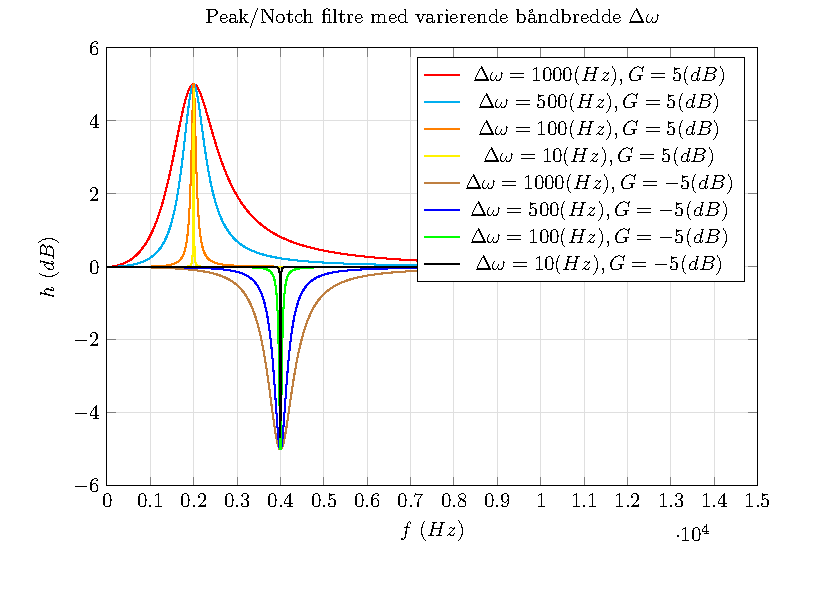
\includegraphics{figure/iir_peak.pdf}
        \caption{Peak/notch filtre med centerfrekvens $f_0 = 2kHz$ og $f_0 = 4kHz$, varierende $Q$ og gain $G=5dB$}
        \label{fig:iir_peak}   
    \end{figure} 
\FloatBlock

     \subsection{Low-shelf filter}

   %  \begin{align}
    %     H_{LS}(z) = \dfrac{\sqrt{G} \left( \sqrt{G} \Omega^2 + \sqrt{2} \Omega G^{\frac{1}{4}} + 1 \right) +2 \sqrt{G} \left( \sqrt{G} \Omega^2 - 1\right) z^{-1} + \sqrt{G} \left(\sqrt{G} \Omega^2- \sqrt{2} \Omega G^{\frac{1}{4}} + 1 \right) z^{-2}}{\sqrt{G} + \sqrt{2} \Omega G^{\frac{1}{4}} + \Omega^2 + 2 \left( \Omega^2 - \sqrt{G} \right) z^{-1} + \left(\sqrt{G} -\sqrt{2} G^{\frac{1}{4}} + \Omega^2 \right) z^{-2}}
    % \end{align}
	
	For at komme fra overføringsfunktionen for peak / notch filteret (\ref{eq:iir_peak_tfz}) til et low shelf filter, sættes $\omega_0 = 0$, for at få de led med $\omega_0$ til at udgå fra ligningen. 
	Forstærkningen ved knækfrekvensen $G_C$ defineres ligeledes $G_B$ i peak/notch filteret.
    Heraf kommer udtrykket for $\beta$, som ses i ligning \ref{eq_iir_beta}.
    \begin{align}
        H_a (s) &= \dfrac{G_0 s + G \beta}{s + \beta} \nonumber \\
        |H_a (\Omega)|^2 &= \dfrac{G_0^2 \Omega^2 + G^2 \beta^2}{\Omega^2 + \beta^2} = G_C^2 \nonumber \\
        \beta &= \sqrt{\dfrac{G_C^2 - G_0^2}{G^2 - G_C^2}} \tan \left( \dfrac{\omega_c}{2} \right) \label{eq_iir_beta}
    \end{align}
	Herefter indsættes $\beta$ i overføringsfunktionen for low shelf filteret og opskrives i ligning \ref{iir_low_shelf}.
     \begin{align}
      H_{LS}(z) =   \dfrac{\left(\dfrac{G_0 + G \beta}{1 + \beta} \right)+ \left(\dfrac{ G_0 - G \beta}{1 + \beta }\right) z^{-1}}{1 + \left( \dfrac{1 - \beta}{1 + \beta} \right) z^{-1}} \label{iir_low_shelf}
     \end{align}
	Lowshelf filteret er plottet i figur \ref{fig:iir_low_shelf} med variende gain, $G$.
%    \begin{figure}[h]
%    \centering
%        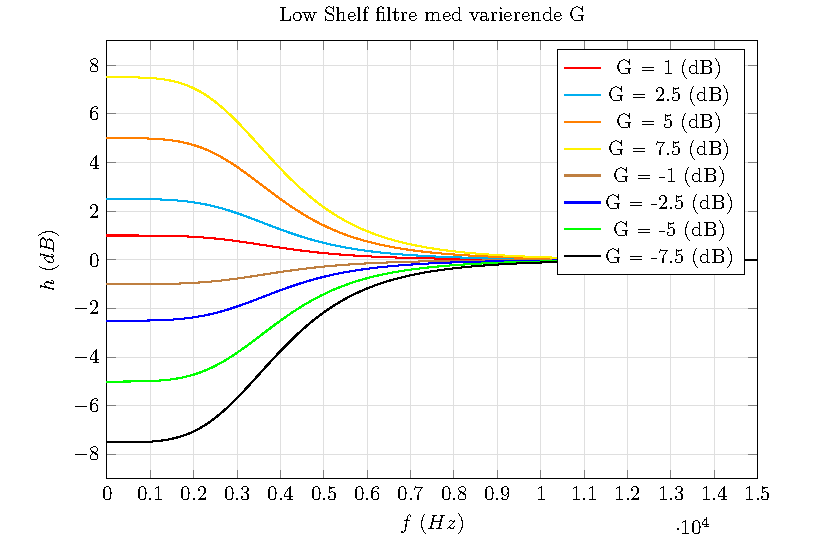
\includegraphics{figure/iir_ls.pdf}
%        \caption{Low shelf filter med knækfrekvens $f_c = 4kHz$, varierende gain $G$ i intervallet: $[-7.5 ; 7.5]$} \label{fig:iir_low_shelf_test}
%    \end{figure}
%	\FloatBlock 
   
   
     \subsection{High-shelf filter}
	I et high shelf filter tages der ligesom i low shelf filteret udgangspunkt i ligning \ref{eq:iir_peak_tfz}. Modsat low shelf filteret sættes $\omega_0 = \pi$.
	Overføringsfunktionen for high shelf filterets opskrives i ligning \ref{iir_hs_tf}.
     \begin{align}
        H_a (s) = \dfrac{G_0 + G \beta s}{1 + \beta s} \label{iir_hs_tf}
     \end{align}
	I ligning \ref{iir_hs_tf_size} findes størrelsen af amplituderne.
     \begin{align}
         |H_a(\Omega)|^2 = \dfrac{G_0^2 + G^2 \beta^2 \Omega^2}{1 + \beta^2 \Omega^2} = G_C^2 \label{iir_hs_tf_size}
     \end{align}
     For at simplificere udtrykket, laves en omskrivning i ligning \ref{iir_beta_helper}. Her indføres knækfrekvensen $\omega_c = \pi - w_0$ og $\omega_0 = \pi$ hvilket vil sætte centerfrekvensen i $f = \infty$, båndbredden bliver heraf knækfrekvensen til high shelf filteret.
    \begin{align}
        \beta = \sqrt{\dfrac{G_C^2 - G_0^2}{G^2 - G_C^2}} \tan \left( \dfrac{\pi - \omega_c}{2} \right) \label{iir_beta_helper}
    \end{align}

    %  \begin{align}
     %    H_{HS} = \dfrac{\sqrt{G} \left(  \sqrt{G} + \sqrt{2} \Omega G^{\frac{1}{4}}+ \Omega^2 \right) -2 \sqrt{G} \left( \sqrt{G} - \Omega^2 \right) z^{-1} + \sqrt{G} \left(\sqrt{G} - \sqrt{2} \Omega G^{\frac{1}{4}} + 1 \right) z^{-2} }{arg}
     %\end{align}


     For at beregne $\beta$ anvendes ligning (\ref{eq:beta}), hvorefter $cos(\omega_0) = cos(\pi) = -1$. Dette giver overføringsfuntionen for high shelf filteret som ses i ligning \ref{iir_hs_tf_zd}, og er en forkortet udgave peak/notch filtrenes overføringsfuntion. Et plot af high shelf filteret ses i figur \ref{fig:iir_high_shelf}
     \begin{align}
     H_{HS}(z) =     \dfrac{\left(\dfrac{G_0 + G \beta}{1 + \beta} \right) + \left(\dfrac{ G_0 - G \beta}{1 + \beta }\right) z^{-1}}{1  + \left( \dfrac{1 - \beta}{1 + \beta} \right) z^{-1}} \label{iir_hs_tf_z}
     \end{align}
%
%
% \begin{figure}[h]
%      \centering
%        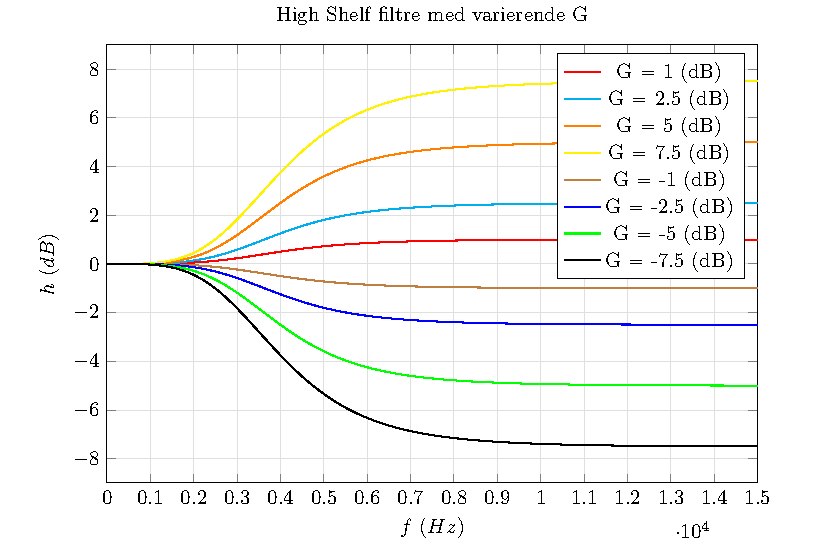
\includegraphics[]{figure/iir_hs.pdf}
%        \caption{High shelf filter med knækfrekvens $f_c = 4kHz$, varierende gain $G$ i intervallet: $[-7.5 ; 7.5]$} \label{fig:iir_high_shelf}
%   \end{figure}  


\begin{figure}[h]
	\centering
	\subbottom[]{%
		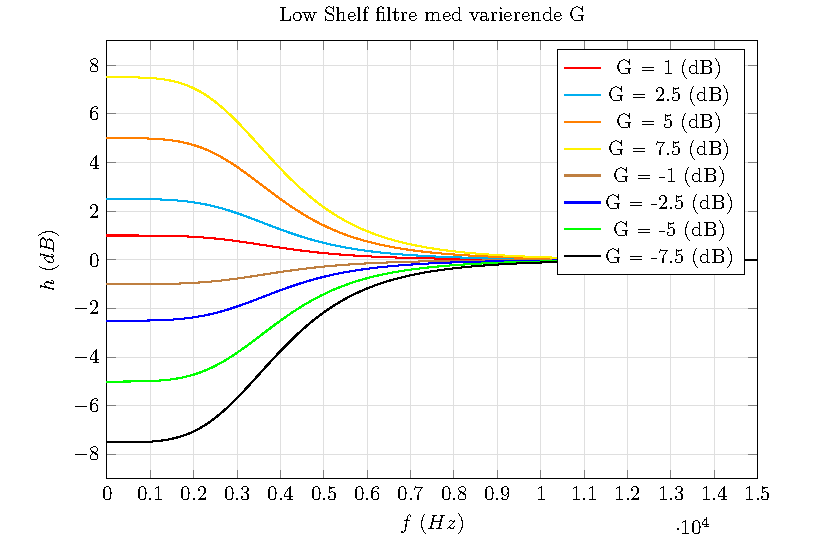
\includegraphics[width=7.35cm]{figure/iir_ls.pdf}
		\label{fig:iir_low_shelf}}
	\subbottom[]{%
		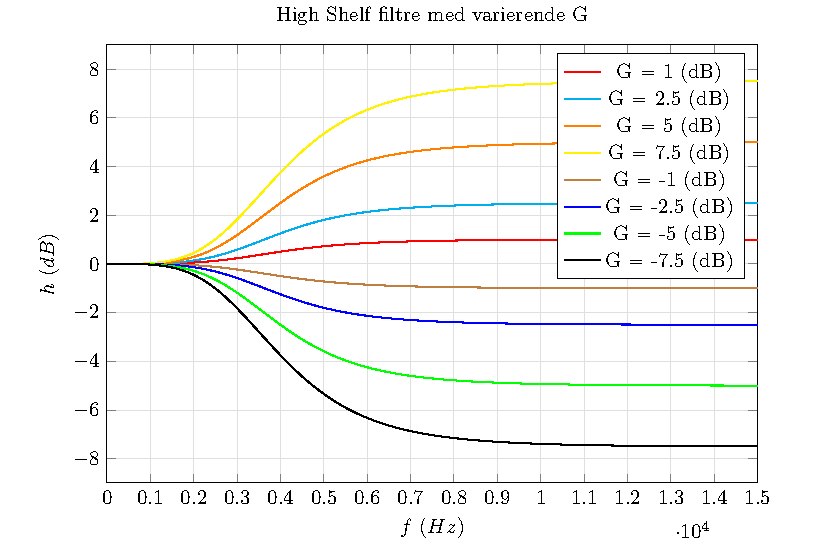
\includegraphics[width=7.35cm]{figure/iir_hs.pdf}
		\label{fig:iir_high_shelf}}
	\caption{\ref{fig:iir_low_shelf}: Low shelf filter. \hspace{4cm} \ref{fig:iir_high_shelf}: High shelf filter. \newline Begge filtre har en knækfrekvensen $f_c = 4kHz$ og et gain $G$ i intervallet: $[-7.5 ; 7.5]$}
\end{figure}
\FloatBlock

\subsection{Fejl ved Bilinear Transformation}


\section{Realisering af filter}

    Differensligning:
    \begin{align}
    y(n) = \sum\limits_{i=0}^{M} b_i x(n-i) - \sum\limits_{i=1}^N a_i y(n-i)
    \end{align}

   %\begin{figure}[h]
        %\centering
        %

\tikzstyle{dspsquare} = [shape=rectangle,draw=black,align=center,text depth=0.3em,text height=1em,inner sep=0pt,
	line cap=round,line join=round,line width=\dspblocklinewidth,minimum size=\dspsquareblocksize]
\tikzstyle{dspmultiplier} = [regular polygon, regular polygon sides=3,align=center,text depth=0.3em,
              text height=1em,inner sep=0mm,
              draw, fill=white, line width=\dspblocklinewidth,     
              shape border rotate=-90]
\tikzstyle{dspadder} = [circle,draw=black, line width=\dspblocklinewidth] 




\begin{tikzpicture}[]

\matrix[column sep=5mm, row sep= 1mm] at (0,0)
{
    %------------------------------------------------------- 
 \node[]               (m00)   {$x(n)$};        &
 \node[dspadder]         (m01)     {$+$} ;     &
 \node[coordinate]             (m02)   {}; &
 \node[coordinate]               (m03)   {};&
\node[coordinate]               (m04)      {}; &
 \node[dspmultiplier]    (m05)       {$ \quad b_0 $};         &
 \node[coordinate]               (m06)       {}; &
 \node[dspadder]         (m07)       {$+$};    &
 \node[]               (m08)        {$y(n)$}; \\ 
%------------------------------------------------------- 
 \node[coordinate]               (m10)       {};        &
 \node[coordinate]               (m11)       {}; &
 \node[coordinate]                (m12)  {}; &
 \node[coordinate]   (m13) {}; &
 \node[dspsquare]         (m14)       {$z^{-1}$};     &
\node[coordinate]        (m15)       {};         &
 \node[coordinate]               (m16)        {}; \\ 
%------------------------------------------------------- 
\node[coordinate]         (m20)       { };            &
\node[coordinate]         (m21)        {}; &
\node[coordinate]         (m22)        {}; &
\node[dspmultiplier,shape border rotate=90]  (m23)    {$-a_1$}; &
\node[coordinate]         (m24)       {};     &
\node[dspmultiplier]     (m25)       {$\quad b_1$};           &
\node[coordinate]       (m26)       { };             \\   
%------------------------------------------------------- 
\node[coordinate]         (m30)       { };            &
\node[coordinate]         (m31)        {}; &
\node[coordinate]         (m32)        {}; &
\node[coordinate]  (m33)    {}; &
\node[dspsquare]         (m34)       {$z^{-1}$};     &
\node[coordinate]      (m35)       {};           &
\node[coordinate]       (m36)       { };             \\  
%------------------------------------------------------- 
\node[coordinate]         (m40)       { };            &
\node[coordinate]         (m41)        {}; &
\node[coordinate]         (m42)        {}; &
\node[dspmultiplier,shape border rotate=90]  (m43)    {$-a_2$}; &
\node[coordinate]        (m44)       {};     &
\node[dspmultiplier]     (m45)       {$\quad b_2$};           &
\node[coordinate]       (m46)       { };             \\    
};

% 1. column
\draw [->] (m00) -- (m01);
\draw [->] (m01) -- (m05);
\draw [->] (m04) node[anchor = south west]{$w[0]$} -- (m14);
\draw [->] (m05) -- (m07);
\draw [->] (m07) -- (m08);
% 2. column
\draw [->] (m14) -- (m24) -- (m25);
\draw [->] (m24) node[anchor =south west]{$w[1]$} -- (m23);
% 3. column
\draw [->] (m24) -- (m34);
\draw [->] (m25) -- (m26) -- (m07);
\draw [->] (m23) -- (m22) -- (m01);

% 4. column
\draw [->] (m34) -- (m44) -- (m45);
\draw [->] (m44)  node[anchor=north west]{$w[2]$} -- (m43);
\draw [->] (m43) -- (m42) -- (m01);
\draw [->] (m45) -- (m46) -- (m07);
\end{tikzpicture}
    %    \caption{Realiserings diagram af 2. ordens iir filter. }    
    %\end{figure}

   



   Koefficienter:\\
   Koefficienterne haves i $K \times 3$ matricer hvor $K$ angiver antal bånd på equalizeren,
    $A_K$ er nævner polynomiet, $B_K$ er tæller polynomiet
   og $W_K$ er state-variablene.  


   \begin{align}
   A_{Kj} = \left[\begin{matrix}
   1 			& a_{01} 	& a_{02} \\
   1 			& a_{11} 	& a_{12} \\
   1 			& a_{21} 	& a_{22} \\
   \vdots 		& \vdots 	&  \vdots \\
   1 			& a_{K1} 	& a_{K2} \\
   \end{matrix}
   \right], \quad
      B_{Kj} = \left[\begin{matrix}
   b_{00}		& b_{01} 	& b_{02} \\
   b_{10}		& b_{11} 	& b_{12} \\
   b_{20}		& b_{21} 	& b_{22} \\
   \vdots 		& \vdots 	&  \vdots \\
   b_{K0}		& b_{K1} 	& b_{K2} \\
   \end{matrix}
   \right], \quad
      w_{Kj} = \left[\begin{matrix}
   w_{00}		& w_{01} 	& w_{02} \\
   w_{10}		& w_{11} 	& w_{12} \\
   w_{20}		& w_{21} 	& w_{22} \\
   \vdots 		& \vdots 	&  \vdots \\
   w_{K0}		& w_{K1} 	& w_{K2} \\
   \end{matrix}
   \right]
   \end{align}
\section{Delkonklusion}

\note{
	Test af CPU og hvordan det er at implementere
}